Lots of dynamics problems are easily solved once we have a set of physical insights about what is happening in the problem. At least, this is the case for the more interesting problems. However, for many AP Physics problems, the way to solve the problem is to recognize the formula that you need to use. It is remarkable how many problems are of the form "imagine that such and such is increased/decreased by a factor of such and such, what happens to such and such?". These problems simply require looking at or recalling the necessary equations and using them. In this section, however, I instead want to focus on some tricks that can help you with more complex problems. The first is to recognize that there are multiple ways of looking at problems. One way is to adopt a "systems approach". It is useful to adopt a systems approach to problems where we have more than one body interacting. This way of thinking can help shorten your calculations significantly and is necessary for more complex problems. By thinking about a group of bodies as a system, I mean to look at all of the bodies as a whole and not to think  about how they are interacting with each other. This is better seen than read, so let us do an example. 

\
\newline
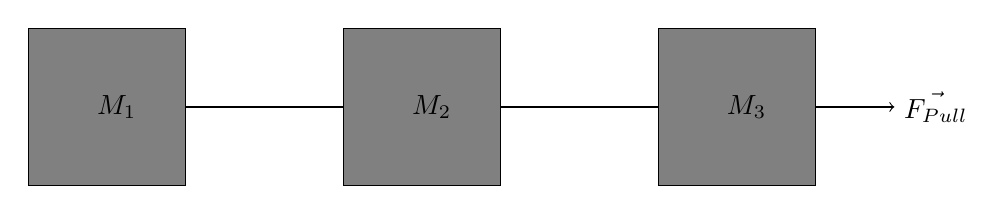
\begin{tikzpicture}

\filldraw[draw= black, fill = gray] (0,0) rectangle (2,2);
\filldraw[draw= black, fill = gray] (4,0) rectangle (6,2);
\filldraw[draw= black, fill = gray] (8,0) rectangle (10,2);
\draw[black] (2,1) -- (4,1);
\draw[black] (6,1) -- (8,1);
\draw[black, ->] (10,1) -- (11,1);
\draw[black] (0.75,1) node[anchor=west] {$M_1$};
\draw[black] (4.75,1) node[anchor=west] {$M_2$};
\draw[black] (8.75,1) node[anchor=west] {$M_3$};
\draw[black] (11,1) node[anchor=west] {$\vec{F_{Pull}}$};
\end{tikzpicture}
\newline
\begin{center}
(Figure 3.9.1)
\end{center}
In Fig. 3.9.1 we see that the three blocks are being pulled by a pulling force. We can imagine that the strings between the blocks are rigid and do not move and are fixed to the blocks. So the blocks are being pulled uniformly. Our task is to find the acceleration of the system. We may assume the rods to be massless. When I first saw a problem like this, I was quite confused. I found it weird that the $M_1$ seemed to have nothing pulling on it but it must have still been moving. However, I was wrong in thinking that there is no force acting on the first $M_1$. The rod between $M_1$ and $M_2$ is pulling on $M_1$ and causing it to move. Additionally, the rod between $M_1$ and $M_2$ is exerting a tension force on $M_2$, but the force is in the opposite direction of $F_{Pull}$. If this confuses you. Think about a small fraction of the rod. It has a net force of 0 acting on it. Why? Because even though it has an acceleration, the mass is 0. So, there is a tension force acting both ways. The same ideas apply for the rod between the 2nd and 3rd masses. We can use Newton’s laws to write equations, and we will be able to find the acceleration, but there is a smarter way. It utilizes the fact that the blocks are moving in parallel, and it is not a particularly complex idea. The simple truth is that we treat the entire mas-rod system as a big system. We can do this because the mass-rod system is connected and will move with one acceleration. We say that $$F_{Pull}=Ma$$ Where $M$ is the mass of the system. Well, what is $M$? Simple, $M$ is just $$M{system} = M_1+M_2+M_3$$ So \begin{equation}a=\frac{F_{Pull}}{M_1+M_2+M_3}\end{equation}. This result makes intuitive sense, if we increase the pulling force, we would expect the acceleration to increase, and it does. Meanwhile, if we increase any of the masses, the acceleration would decrease, which makes sense. Now that we have seen the systems approach I encourage you to solve this problem without using this and compare to see how powerful this method is. Now, if you are still confused, I want you to think about it in the following way. I did not specify how long the rod was. What if it was tiny, only the length of a few atoms. All of the calculations would be the same as we still have the same ideas, but we could think of it as being one extended block of mass $$M_{block}=M_1+M_2+M_3$$ being pulled. From here, we can think about this as being a one body problem because after all, we could arbitrarily split any given mass into smaller masses and we would essentially have a three-body problem. This is a classical example in physics of thinking about the asymptotic behavior of a formula in order to determine its validity.